\documentclass[a4paper]{article}

% - - - - - - -  - - - - - Packages - - - - - - - - - - - - 
\usepackage{amsmath, accents}
\usepackage{amsfonts}                       % Add mathematical symbols and functionality
\usepackage{amssymb}
\usepackage{mathrsfs}                       % More mathematical letters
\usepackage[margin=2.2cm]{geometry}         % Change margins
\usepackage[shortlabels]{enumitem}          % Enumerate things
\usepackage{graphicx}                       % Enables pictures 

%\usepackage[english]{babel}
\usepackage[dutch]{babel}                  % Language settings

\usepackage{float}                          % Force pictures in right place
\usepackage[useregional]{datetime2}         % Use current date 
\usepackage{braket}                         % Make braket notation and sets
\usepackage{interval}                       % Custom intervals in Bourbaki notation
\usepackage{lipsum}                         % Put in sections of Lorem ipsum
\usepackage{amsthm}                         % For theorem and proof environments

\usepackage[all]{xy}                        % Make cummutative diagrams

\usepackage{tikz}                           % Make tikz pictures

\usepackage{hyperref}                       % Make links and references
\usepackage{cleveref}                       % More options for references


% - - - - - - -  - - - - - Theorem environments - - - - - - - 
\newtheorem{stelling}{Stelling}
\newtheorem{gevolg}[stelling]{Gevolg}
\newtheorem{lemma}[stelling]{Lemma}	
\newtheorem{propositie}[stelling]{Propositie}

% - - - - - - -  - - - - - Newcommands - - - - - - - - - - - 
\newcommand{\N}{\mathbb{N}}
\newcommand{\Z}{\mathbb{Z}}
\newcommand{\id}{\mathrm{id}}

\newcommand{\norm}[1]{ \left\| #1 \right\| }

\newcommand{\pointsvector}{\overrightarrow{AB}}

\newcommand{\desda}{dan en slechts dan als }

\renewcommand{\d}{\mathrm{d}}

\newcommand{\HandinTitle}[2]{\DTMsetdatestyle{ddmmyyyy}
\begin{center}
   { \huge #1} \\
   \vspace{4mm}
   \large{#2\\ \today}
   \vspace{4mm}
   \hrule
   \vspace{2mm}
\end{center}}

\begin{document}

\HandinTitle{Inlever template 2}{\TeX niCie}

Dit is een template voor een inleveropgave. 
Dit template heef iets meer functionaliteit dan de simpelere versie.
We hebben heir onze eigen titel gemaakt met een command dat we hiervoor hebben geschreven.
Je kunt alles aanpassen zoals je zelf wil.
We zullen hier wat andere dingen laten zien dan in het simplere template. 

\begin{description}
    \item[Opgave 1.] Dit is opgave 1. 
    Soms wil je dat de tekst onder het opgavenummer komt. Dat kan op de volgende manier: 

    \item[Opgave 2.] \hfill \\
    Dit is opgave 2. We hebben een paar extra newcommands toegevoegd, zoals 
    \desda. 
    De preamble is hierdoor wat langer geworden. 
    We raden aan om deze in een apart document te zetten.
    In een overleaf project kun je meerdere .tex bestanden hebben. 
    Plaats alle packages en newcommands in een andere bestandje, bijvoorbeeld 
    packages.tex. Vervolgens breng je dit naar je main.tex met 
    \texttt{input\{packages.tex\}}. % \input{packages.tex}
    Plaats dit tussen \texttt{documentclass} en \texttt{begin\{document\}}. 

    \item[Opgave 3.] \hfill \\
    We hebben een package toegevoegd voor intervallen. 
    We kunnen nu intervallen maken met \(\interval{a}{b}\).
    Dit ziet er iets beter uit dan \([a,b]\). 
    We kunnen open en half-open intervallen maken als volgt:
    \begin{align*}
        \interval{a}{b} & &\interval[open]{a}{b} \\
        \interval[open left]{a}{b} & &\interval[open right]{a}{b}
    \end{align*}
    Je zult zien dat de spacing hier \(x \in \interval[open]{a}{b}\) 
    beter is dan zonder de package \(x \in ]a,b[ \). Verder 
    kun je ook de haakjes laten schalen: 
    \[ x \in \interval[scaled, open right]{\int_1^\infty \frac{1}{y^3} \d y}{10^5}. \]

    We hebben ook theorem environments toegevoegd, zoals 
    \begin{stelling}
        Dit is een stelling. 
    \end{stelling}
    \begin{proof}
        Het bewijs voor deze stelling is triviaal.
    \end{proof}

    We hebben ook nog de tikz package. 
    Dit kun je gebruiken om plaatjes te maken, zoals dit:

    \begin{figure}[H]
        \centering
        \tikzset{every picture/.style={line width=0.75pt}} %set default line width to 0.75pt        

    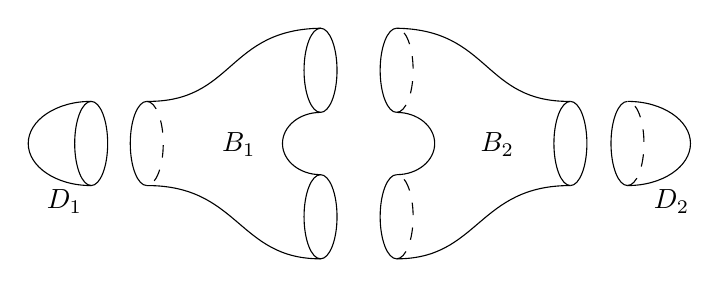
\begin{tikzpicture}[x=0.75pt,y=0.75pt,yscale=-0.5,xscale=0.5]
    %uncomment if require: \path (0,300); %set diagram left start at 0, and has height of 300

    %Shape: Arc [id:dp715273445875235] 
    \draw  [draw opacity=0] (145.89,186.6) .. controls (145.89,186.6) and (145.89,186.6) .. (145.89,186.6) .. controls (137.11,186.6) and (130,168.45) .. (130,146.05) .. controls (130,123.65) and (137.11,105.5) .. (145.89,105.5) -- (145.89,146.05) -- cycle ; \draw   (145.89,186.6) .. controls (145.89,186.6) and (145.89,186.6) .. (145.89,186.6) .. controls (137.11,186.6) and (130,168.45) .. (130,146.05) .. controls (130,123.65) and (137.11,105.5) .. (145.89,105.5) ;  
    %Shape: Ellipse [id:dp5523465046994875] 
    \draw   (297.44,75.55) .. controls (297.44,53.15) and (304.56,35) .. (313.33,35) .. controls (322.11,35) and (329.22,53.15) .. (329.22,75.55) .. controls (329.22,97.95) and (322.11,116.1) .. (313.33,116.1) .. controls (304.56,116.1) and (297.44,97.95) .. (297.44,75.55) -- cycle ;
    %Shape: Ellipse [id:dp15397833647486892] 
    \draw   (297.44,216.65) .. controls (297.44,194.25) and (304.56,176.1) .. (313.33,176.1) .. controls (322.11,176.1) and (329.22,194.25) .. (329.22,216.65) .. controls (329.22,239.05) and (322.11,257.2) .. (313.33,257.2) .. controls (304.56,257.2) and (297.44,239.05) .. (297.44,216.65) -- cycle ;
    %Shape: Arc [id:dp025456778054827045] 
    \draw  [draw opacity=0] (313.33,176.1) .. controls (313.33,176.1) and (313.33,176.1) .. (313.33,176.1) .. controls (313.33,176.1) and (313.33,176.1) .. (313.33,176.1) .. controls (293.08,176.1) and (276.67,162.67) .. (276.67,146.1) .. controls (276.67,129.53) and (293.08,116.1) .. (313.33,116.1) .. controls (313.33,116.1) and (313.33,116.1) .. (313.33,116.1) -- (313.33,146.1) -- cycle ; \draw   (313.33,176.1) .. controls (313.33,176.1) and (313.33,176.1) .. (313.33,176.1) .. controls (313.33,176.1) and (313.33,176.1) .. (313.33,176.1) .. controls (293.08,176.1) and (276.67,162.67) .. (276.67,146.1) .. controls (276.67,129.53) and (293.08,116.1) .. (313.33,116.1) .. controls (313.33,116.1) and (313.33,116.1) .. (313.33,116.1) ;  
    %Curve Lines [id:da017416770248540603] 
    \draw    (145.89,105.5) .. controls (230,106.4) and (223,36.4) .. (313.33,35) ;
    %Curve Lines [id:da05326705201725679] 
    \draw    (145.89,186.6) .. controls (235,186.4) and (234,257.4) .. (313.33,257.2) ;
    %Shape: Arc [id:dp44692039379070725] 
    \draw  [draw opacity=0][dash pattern={on 4.5pt off 4.5pt}] (145.89,105.5) .. controls (145.89,105.5) and (145.89,105.5) .. (145.89,105.5) .. controls (154.66,105.5) and (161.78,123.65) .. (161.78,146.05) .. controls (161.78,168.45) and (154.66,186.6) .. (145.89,186.6) -- (145.89,146.05) -- cycle ; \draw  [dash pattern={on 4.5pt off 4.5pt}] (145.89,105.5) .. controls (145.89,105.5) and (145.89,105.5) .. (145.89,105.5) .. controls (154.66,105.5) and (161.78,123.65) .. (161.78,146.05) .. controls (161.78,168.45) and (154.66,186.6) .. (145.89,186.6) ;  
    %Shape: Arc [id:dp9329343652812118] 
    \draw  [draw opacity=0] (554.11,186.6) .. controls (554.11,186.6) and (554.11,186.6) .. (554.11,186.6) .. controls (562.89,186.6) and (570,168.45) .. (570,146.05) .. controls (570,123.65) and (562.89,105.5) .. (554.11,105.5) -- (554.11,146.05) -- cycle ; \draw   (554.11,186.6) .. controls (554.11,186.6) and (554.11,186.6) .. (554.11,186.6) .. controls (562.89,186.6) and (570,168.45) .. (570,146.05) .. controls (570,123.65) and (562.89,105.5) .. (554.11,105.5) ;  
    %Shape: Arc [id:dp7533250478247696] 
    \draw  [draw opacity=0] (386.67,35) .. controls (386.67,35) and (386.67,35) .. (386.67,35) .. controls (377.89,35) and (370.78,53.15) .. (370.78,75.55) .. controls (370.78,97.95) and (377.89,116.1) .. (386.67,116.1) -- (386.67,75.55) -- cycle ; \draw   (386.67,35) .. controls (386.67,35) and (386.67,35) .. (386.67,35) .. controls (377.89,35) and (370.78,53.15) .. (370.78,75.55) .. controls (370.78,97.95) and (377.89,116.1) .. (386.67,116.1) ;  
    %Shape: Arc [id:dp6251510904362046] 
    \draw  [draw opacity=0] (386.67,176.1) .. controls (386.67,176.1) and (386.67,176.1) .. (386.67,176.1) .. controls (377.89,176.1) and (370.78,194.25) .. (370.78,216.65) .. controls (370.78,239.05) and (377.89,257.2) .. (386.67,257.2) -- (386.67,216.65) -- cycle ; \draw   (386.67,176.1) .. controls (386.67,176.1) and (386.67,176.1) .. (386.67,176.1) .. controls (377.89,176.1) and (370.78,194.25) .. (370.78,216.65) .. controls (370.78,239.05) and (377.89,257.2) .. (386.67,257.2) ;  
    %Shape: Arc [id:dp3417277016359854] 
    \draw  [draw opacity=0] (386.67,176.1) .. controls (386.67,176.1) and (386.67,176.1) .. (386.67,176.1) .. controls (406.92,176.1) and (423.33,162.67) .. (423.33,146.1) .. controls (423.33,129.53) and (406.92,116.1) .. (386.67,116.1) -- (386.67,146.1) -- cycle ; \draw   (386.67,176.1) .. controls (386.67,176.1) and (386.67,176.1) .. (386.67,176.1) .. controls (406.92,176.1) and (423.33,162.67) .. (423.33,146.1) .. controls (423.33,129.53) and (406.92,116.1) .. (386.67,116.1) ;  
    %Curve Lines [id:da28998933316772246] 
    \draw    (554.11,105.5) .. controls (470,106.4) and (477,36.4) .. (386.67,35) ;
    %Curve Lines [id:da7166122915889644] 
    \draw    (554.11,186.6) .. controls (465,186.4) and (466,257.4) .. (386.67,257.2) ;
    %Shape: Arc [id:dp21244976427938544] 
    \draw  [draw opacity=0] (554.11,105.5) .. controls (554.11,105.5) and (554.11,105.5) .. (554.11,105.5) .. controls (545.34,105.5) and (538.22,123.65) .. (538.22,146.05) .. controls (538.22,168.45) and (545.34,186.6) .. (554.11,186.6) -- (554.11,146.05) -- cycle ; \draw   (554.11,105.5) .. controls (554.11,105.5) and (554.11,105.5) .. (554.11,105.5) .. controls (545.34,105.5) and (538.22,123.65) .. (538.22,146.05) .. controls (538.22,168.45) and (545.34,186.6) .. (554.11,186.6) ;  
    %Shape: Arc [id:dp03596106482590211] 
    \draw  [draw opacity=0][dash pattern={on 4.5pt off 4.5pt}] (386.67,116.1) .. controls (386.67,116.1) and (386.67,116.1) .. (386.67,116.1) .. controls (386.67,116.1) and (386.67,116.1) .. (386.67,116.1) .. controls (395.44,116.1) and (402.56,97.95) .. (402.56,75.55) .. controls (402.56,53.15) and (395.44,35) .. (386.67,35) -- (386.67,75.55) -- cycle ; \draw  [dash pattern={on 4.5pt off 4.5pt}] (386.67,116.1) .. controls (386.67,116.1) and (386.67,116.1) .. (386.67,116.1) .. controls (386.67,116.1) and (386.67,116.1) .. (386.67,116.1) .. controls (395.44,116.1) and (402.56,97.95) .. (402.56,75.55) .. controls (402.56,53.15) and (395.44,35) .. (386.67,35) ;  
    %Shape: Arc [id:dp10974079301350659] 
    \draw  [draw opacity=0][dash pattern={on 4.5pt off 4.5pt}] (386.67,257.2) .. controls (386.67,257.2) and (386.67,257.2) .. (386.67,257.2) .. controls (386.67,257.2) and (386.67,257.2) .. (386.67,257.2) .. controls (395.44,257.2) and (402.56,239.05) .. (402.56,216.65) .. controls (402.56,194.25) and (395.44,176.1) .. (386.67,176.1) -- (386.67,216.65) -- cycle ; \draw  [dash pattern={on 4.5pt off 4.5pt}] (386.67,257.2) .. controls (386.67,257.2) and (386.67,257.2) .. (386.67,257.2) .. controls (386.67,257.2) and (386.67,257.2) .. (386.67,257.2) .. controls (395.44,257.2) and (402.56,239.05) .. (402.56,216.65) .. controls (402.56,194.25) and (395.44,176.1) .. (386.67,176.1) ;  
    %Shape: Ellipse [id:dp3805875981770903] 
    \draw   (76.44,146.05) .. controls (76.44,123.65) and (83.56,105.5) .. (92.33,105.5) .. controls (101.11,105.5) and (108.22,123.65) .. (108.22,146.05) .. controls (108.22,168.45) and (101.11,186.6) .. (92.33,186.6) .. controls (83.56,186.6) and (76.44,168.45) .. (76.44,146.05) -- cycle ;
    %Shape: Arc [id:dp6558849275533489] 
    \draw  [draw opacity=0] (92.35,186.6) .. controls (92.25,186.6) and (92.15,186.6) .. (92.05,186.6) .. controls (58.7,186.6) and (31.67,168.45) .. (31.67,146.05) .. controls (31.67,123.65) and (58.7,105.5) .. (92.05,105.5) -- (92.05,146.05) -- cycle ; \draw   (92.35,186.6) .. controls (92.25,186.6) and (92.15,186.6) .. (92.05,186.6) .. controls (58.7,186.6) and (31.67,168.45) .. (31.67,146.05) .. controls (31.67,123.65) and (58.7,105.5) .. (92.05,105.5) ;  
    %Shape: Arc [id:dp5924304365469244] 
    \draw  [draw opacity=0] (609.11,105.5) .. controls (609.11,105.5) and (609.11,105.5) .. (609.11,105.5) .. controls (600.34,105.5) and (593.22,123.65) .. (593.22,146.05) .. controls (593.22,168.45) and (600.34,186.6) .. (609.11,186.6) -- (609.11,146.05) -- cycle ; \draw   (609.11,105.5) .. controls (609.11,105.5) and (609.11,105.5) .. (609.11,105.5) .. controls (600.34,105.5) and (593.22,123.65) .. (593.22,146.05) .. controls (593.22,168.45) and (600.34,186.6) .. (609.11,186.6) ;  
    %Shape: Arc [id:dp8600055157420703] 
    \draw  [draw opacity=0][dash pattern={on 4.5pt off 4.5pt}] (609.11,186.6) .. controls (609.11,186.6) and (609.11,186.6) .. (609.11,186.6) .. controls (617.89,186.6) and (625,168.45) .. (625,146.05) .. controls (625,123.65) and (617.89,105.5) .. (609.11,105.5) -- (609.11,146.05) -- cycle ; \draw  [dash pattern={on 4.5pt off 4.5pt}] (609.11,186.6) .. controls (609.11,186.6) and (609.11,186.6) .. (609.11,186.6) .. controls (617.89,186.6) and (625,168.45) .. (625,146.05) .. controls (625,123.65) and (617.89,105.5) .. (609.11,105.5) ;  
    %Shape: Arc [id:dp1536964284250496] 
    \draw  [draw opacity=0] (609.11,186.6) .. controls (609.21,186.6) and (609.31,186.6) .. (609.41,186.6) .. controls (642.77,186.6) and (669.81,168.45) .. (669.81,146.05) .. controls (669.81,123.66) and (642.77,105.5) .. (609.41,105.5) -- (609.41,146.05) -- cycle ; \draw   (609.11,186.6) .. controls (609.21,186.6) and (609.31,186.6) .. (609.41,186.6) .. controls (642.77,186.6) and (669.81,168.45) .. (669.81,146.05) .. controls (669.81,123.66) and (642.77,105.5) .. (609.41,105.5) ;  

    % Text Node
    \draw (47,188.4) node [anchor=north west][inner sep=0.75pt]    {$D_{1}$};
    % Text Node
    \draw (216,133.4) node [anchor=north west][inner sep=0.75pt]    {$B_{1}$};
    % Text Node
    \draw (465,133.4) node [anchor=north west][inner sep=0.75pt]    {$B_{2}$};
    % Text Node
    \draw (632,188.4) node [anchor=north west][inner sep=0.75pt]    {$D_{2}$};


    \end{tikzpicture}
    \caption{Een torus in stukjes opgehakt}
    \label{fig:torus}
    \end{figure}




    We raden sterk af om dit soort plaatjes handmatig te schrijven, 
    \cref{fig:torus} was gemaakt via \url{https://www.mathcha.io/editor}.


\end{description}

\end{document}